% 第 2 章 双曲不动点与 Koenigs 坐标
% 经典部分：Koenigs 1884；Milnor 2006 §8；Carleson--Gamelin Ch. II。
% 本理论部分：[KneserPaper] §2.1（Lemma param）、§3.1（S、R^{-1} 与 Lemma realT）、sec-general.tex（(H4) 的改写）。
% 数值：figures/ch02_sqrt2.py；图：figures/fig2_regular.py。
\chapter{双曲不动点与 Koenigs 坐标}\label{ch:koenigs}

本章讲两个不动点中「容易」的那一类：乘子 $\lambda$ 满足 $|\lambda|\ne0,1$ 的不动点。
在这样的不动点附近，映射可以全纯地共轭成乘法 $\zeta\mapsto\lambda\zeta$（Koenigs 定理），
共轭坐标在相差常数倍的意义下唯一。对它取对数再除以 $\log\lambda$，就得到 Abel 坐标；
它的逆是一个超函数，即「正则迭代」。

本章后半部分把这些经典事实用到一个具体设定上：实轴上的实映射 $f$，有相邻的吸引不动点 $u_1$ 和排斥不动点 $u_2$。
两个不动点各给出一个超函数，记作 $R$ 和 $S$（\cref{def:regular-solution}）。
它们是全书的两块基本材料：第~\ref{ch:transition}~章用它们定义转移映射，第~\ref{ch:sewing}~章把它们缝起来。
本章的例子是 $b^w$（$1<b<\eta$），算例取 $b=\sqrt2$。

\begin{goals}
\item Koenigs 线性化定理（\cref{thm:koenigs}）的完整证明，以及 Schröder 映射在相差常数倍意义下的唯一性（\cref{ch2:cor:schroder-unique}）。
\item 吸引不动点的 Koenigs 坐标沿函数方程延拓到整个吸引域；排斥不动点的 Poincaré 函数延拓为整函数（\cref{ch2:prop:extend,ch2:prop:poincare}）。
\item 实映射的两个正则解 $R$、$S$（\cref{def:regular-solution}）：它们有虚周期 $\ii h$、$\ii h_2$，在实轴上有确定的实结构（\cref{prop:regular-periodic}），并由「在半平面上一致收敛到不动点」刻画（\cref{ch2:prop:regular-unique}）。
\item $R$ 与 $S$ 在区间 $(u_1,u_2)$ 上给出两个不同的实解析分数次迭代；它们的差就是第~\ref{ch:transition}~章的转移映射。$b=\sqrt2$ 时两者相差约 $10^{-25}$（\cref{ch2:ex:sqrt2-transition}）。
\end{goals}

% ==================================================================
\section{线性化问题}\label{ch2:sec:linearization}

设 $f$ 在点 $p$ 的邻域内全纯，$f(p)=p$。称 $\lambda:=f'(p)$ 为不动点 $p$ 的\textbf{乘子}（multiplier）。按 $\lambda$ 分类：
\begin{itemize}
\item $\lambda=0$：\textbf{超吸引}（superattracting）；
\item $0<|\lambda|<1$：\textbf{吸引}（attracting）；
\item $|\lambda|>1$：\textbf{排斥}（repelling）；
\item $|\lambda|=1$：\textbf{中性}（neutral），其中 $\lambda$ 为单位根时称为\textbf{抛物}（parabolic）。
\end{itemize}
本章处理 $0<|\lambda|<1$ 与 $|\lambda|>1$ 两种情形，统称\textbf{双曲}（hyperbolic）不动点。
抛物情形 $\lambda=1$ 是第~\ref{ch:fatou}~章的主题。

\textbf{线性化问题}是：是否存在 $p$ 附近的全纯函数 $\sigma$，$\sigma(p)=0$，$\sigma'(p)=1$，使
\begin{equation}\label{ch2:eq:schroder}
  \sigma\circ f=\lambda\,\sigma .
\end{equation}
这就是第~\ref{ch:intro}~章的 Schröder 方程，满足它的 $\sigma$ 称为 \textbf{Schröder 映射}（Schröder map）或 \textbf{Koenigs 坐标}（Koenigs coordinate）。
若 $\sigma$ 存在，则它在 $p$ 附近单叶，并且 $f=\sigma^{-1}\circ(\lambda\,\cdot)\circ\sigma$：在坐标 $\zeta=\sigma(u)$ 中，$f$ 就是乘以 $\lambda$。

先看形式层面。不妨设 $p=0$。

\begin{lemma}[形式解]\label{ch2:lem:formal}
设 $f(z)=\lambda z+\sum_{k\ge2}f_kz^k$ 是形式幂级数，$\lambda\ne0$，且 $\lambda^{k-1}\ne1$ 对一切 $k\ge2$ 成立。
则存在唯一的形式幂级数 $\sigma(z)=z+\sum_{k\ge2}s_kz^k$ 使 $\sigma\circ f=\lambda\sigma$。系数由递推
\begin{equation}\label{ch2:eq:recursion}
  (\lambda-\lambda^k)\,s_k=\bigl[z^k\bigr]\Bigl(f(z)+\sum_{j=2}^{k-1}s_j\,f(z)^j\Bigr)\qquad(k\ge2)
\end{equation}
确定，其中 $[z^k]$ 表示取 $z^k$ 的系数。
\end{lemma}

\begin{proof}
$\sigma(f(z))=f(z)+\sum_{j\ge2}s_jf(z)^j$。因为 $f(z)^j=\lambda^jz^j+O(z^{j+1})$，
$z^k$ 的系数中含 $s_k$ 的项只有 $s_k\lambda^k$，其余项只含 $s_2,\dots,s_{k-1}$。
比较 $\sigma\circ f$ 与 $\lambda\sigma$ 的 $z^k$ 系数，得到 $\lambda^ks_k+[z^k](f+\sum_{j<k}s_jf^j)=\lambda s_k$，即 \eqref{ch2:eq:recursion}。
因为 $\lambda-\lambda^k=\lambda(1-\lambda^{k-1})\ne0$，$s_k$ 被唯一确定。
\end{proof}

当 $0<|\lambda|<1$ 或 $|\lambda|>1$ 时，$|\lambda^{k-1}|\ne1$，条件自动成立，并且分母 $|\lambda-\lambda^k|$ 远离零：
$0<|\lambda|<1$ 时 $|\lambda-\lambda^k|\ge|\lambda|(1-|\lambda|)$。这正是收敛的原因。
当 $|\lambda|=1$ 而 $\lambda$ 不是单位根时，分母可以任意小（「小分母」），收敛与否取决于 $\lambda$ 的辐角的算术性质（Siegel、Brjuno、Cremer，见~\cite[\S11]{Milnor2006}）。
当 $\lambda=1$ 时递推在 $k=2$ 就失效：抛物不动点不能线性化，取而代之的是 Fatou 坐标（第~\ref{ch:fatou}~章）。

% ==================================================================
\section{Koenigs 线性化定理}\label{ch2:sec:koenigs}

\begin{theorem}[Koenigs~\cite{Koenigs1884}]\label{thm:koenigs}
设 $f$ 在 $p$ 的邻域内全纯，$f(p)=p$，$\lambda=f'(p)$ 满足 $0<|\lambda|<1$ 或 $|\lambda|>1$。则存在 $p$ 的邻域 $U$ 和 $U$ 上的单叶全纯函数 $\sigma$，使
\[
  \sigma(p)=0,\qquad \sigma'(p)=1,\qquad \sigma(f(u))=\lambda\,\sigma(u)\quad(u\in U\cap f^{-1}(U)).
\]
满足这三个条件的全纯函数芽是唯一的。吸引情形下可以取 $U$ 使 $f(U)\subset U$，并且
\begin{equation}\label{ch2:eq:koenigs-limit}
  \sigma(u)=\lim_{n\to\infty}\lambda^{-n}\bigl(f^{\circ n}(u)-p\bigr)
\end{equation}
在 $U$ 上一致成立。
\end{theorem}

\begin{proof}
不妨设 $p=0$。

\emph{吸引情形 $0<|\lambda|<1$。}
取常数 $c$ 使 $|\lambda|<c<\sqrt{|\lambda|}$（这是可能的，因为 $|\lambda|<1$ 推出 $|\lambda|<\sqrt{|\lambda|}$）。
由 Taylor 展开，存在 $r_0>0$、$C>0$ 使
\begin{equation}\label{ch2:eq:taylor}
  |f(z)-\lambda z|\le C|z|^2\qquad(|z|\le r_0).
\end{equation}
取 $0<r\le r_0$ 使 $|\lambda|+Cr\le c$。则对 $|z|\le r$ 有 $|f(z)|\le(|\lambda|+C|z|)|z|\le c|z|$，
所以 $f$ 把闭圆盘 $\overline D_r=\{|z|\le r\}$ 映入自身，且
\begin{equation}\label{ch2:eq:orbit-bound}
  |f^{\circ n}(z)|\le c^n|z|\qquad(|z|\le r,\ n\ge0).
\end{equation}
令 $\sigma_n(z):=\lambda^{-n}f^{\circ n}(z)$。由 \eqref{ch2:eq:taylor}、\eqref{ch2:eq:orbit-bound}，
\[
  |\sigma_{n+1}(z)-\sigma_n(z)|
  =|\lambda|^{-n-1}\bigl|f(f^{\circ n}(z))-\lambda f^{\circ n}(z)\bigr|
  \le|\lambda|^{-n-1}C\,|f^{\circ n}(z)|^2
  \le\frac{Cr^2}{|\lambda|}\Bigl(\frac{c^2}{|\lambda|}\Bigr)^{n}.
\]
因为 $c^2<|\lambda|$，级数 $\sum_n(\sigma_{n+1}-\sigma_n)$ 在 $\overline D_r$ 上一致收敛，
所以 $\sigma_n$ 一致收敛到 $D_r$ 上的全纯函数 $\sigma$，这就是 \eqref{ch2:eq:koenigs-limit}。
每个 $\sigma_n$ 满足 $\sigma_n(0)=0$、$\sigma_n'(0)=1$，取极限得 $\sigma(0)=0$、$\sigma'(0)=1$。
又 $\sigma_n(f(z))=\lambda\sigma_{n+1}(z)$，取极限得 $\sigma\circ f=\lambda\sigma$ 于 $D_r$。
$\sigma'(0)\ne0$，所以 $\sigma$ 在 $0$ 的某个邻域上单叶；
取 $U$ 为该邻域中的一个小圆盘 $D_{r'}$（$r'\le r$），则 $f(U)\subset U$ 仍成立。

唯一性：设 $\varphi$ 在 $D_\rho$ 上全纯，$\varphi(0)=0$，$\varphi'(0)=1$，并在 $0$ 附近满足 $\varphi\circ f=\lambda\varphi$。
缩小 $r$（上面关于 $r$ 的条件对更小的 $r$ 仍成立），可设 $r\le\rho$，$\varphi\circ f=\lambda\varphi$ 于 $D_r$，并且 $|\varphi(w)-w|\le M|w|^2$（$|w|\le r$）。
因为 $f^{\circ n}(D_r)\subset D_r$，迭代函数方程得 $\varphi=\lambda^{-n}\varphi\circ f^{\circ n}$ 于 $D_r$，于是
\[
  |\varphi(z)-\sigma_n(z)|=|\lambda|^{-n}\bigl|\varphi(f^{\circ n}(z))-f^{\circ n}(z)\bigr|
  \le|\lambda|^{-n}M|f^{\circ n}(z)|^2\le Mr^2\Bigl(\frac{c^2}{|\lambda|}\Bigr)^n\to0 .
\]
所以 $\varphi=\lim\sigma_n=\sigma$ 于 $D_r$。

\emph{排斥情形 $|\lambda|>1$。}
$f'(0)=\lambda\ne0$，所以 $f$ 把 $0$ 的某个邻域 $U_0$ 双全纯地映到 $0$ 的邻域 $V_0$。
记 $\iota:=(f|_{U_0})^{-1}:V_0\to U_0$，则 $\iota(0)=0$，$\iota'(0)=1/\lambda$，$0<|1/\lambda|<1$。
对 $\iota$ 用吸引情形，得到 $0$ 附近的单叶函数 $\sigma$，$\sigma(0)=0$，$\sigma'(0)=1$，$\sigma\circ \iota=\lambda^{-1}\sigma$。
对 $u$ 靠近 $0$，令 $w=f(u)$，则 $\iota(w)=u$，上式给出 $\sigma(u)=\lambda^{-1}\sigma(f(u))$，即 $\sigma\circ f=\lambda\sigma$。
反过来，$0$ 附近满足 $\sigma\circ f=\lambda\sigma$ 的函数也满足 $\sigma\circ \iota=\lambda^{-1}\sigma$，所以唯一性由吸引情形推出。
\end{proof}

\begin{corollary}[Schröder 映射的唯一性]\label{ch2:cor:schroder-unique}
在 \cref{thm:koenigs} 的条件下，设 $\varphi$ 在 $p$ 附近全纯，$\varphi(p)=0$，且 $\varphi\circ f=\lambda\varphi$。则 $\varphi=\varphi'(p)\,\sigma$。
特别地，满足 \eqref{ch2:eq:schroder} 且在 $p$ 处为零的全纯函数，在相差一个常数倍的意义下唯一。
\end{corollary}

\begin{proof}
若 $\varphi'(p)\ne0$，对 $\varphi/\varphi'(p)$ 用 \cref{thm:koenigs} 的唯一性。
若 $\varphi'(p)=0$ 而 $\varphi\not\equiv0$，设 $\varphi(u)=a_m(u-p)^m+O((u-p)^{m+1})$，$m\ge2$，$a_m\ne0$。
比较 $\varphi(f(u))=a_m\lambda^m(u-p)^m+\cdots$ 与 $\lambda\varphi(u)=\lambda a_m(u-p)^m+\cdots$ 的首项，得 $\lambda^{m-1}=1$，与 $|\lambda|\ne1$ 矛盾。
\end{proof}

\begin{remark}[实结构]\label{ch2:rem:real-sigma}
设 $f$ 在实轴上取实值（即 $f(\bar u)=\overline{f(u)}$），$p$ 与 $\lambda$ 为实数。
则 $\tilde\sigma(u):=\overline{\sigma(\bar u)}$ 也满足 \cref{thm:koenigs} 的三个条件，由唯一性 $\tilde\sigma=\sigma$。
所以 $\sigma$ 在实轴上取实值。若 $\lambda>0$ 且 $\sigma'(p)=1$，则 $\sigma$ 在 $p$ 附近的实轴上严格递增。
\end{remark}

\begin{remark}[关于引用]\label{ch2:rem:koenigs-references}
上面的证明沿用 Koenigs 的原始思路（$\sigma=\lim\lambda^{-n}f^{\circ n}$），与~\cite[\S8，Theorem~8.2]{Milnor2006} 和~\cite[Ch.~II]{CarlesonGamelin1993} 的处理相同。
唯一性的证明直接用极限，不需要比较幂级数系数。
\end{remark}

% ==================================================================
\section{整体延拓}\label{ch2:sec:global}

Koenigs 坐标起初只在 $p$ 的一个小邻域内有定义。函数方程 \eqref{ch2:eq:schroder} 把它延拓到大得多的区域。
本节设 $f:\Omega\to\Omega$ 在区域 $\Omega\subset\C$ 上全纯；本书的例子中 $\Omega=\C$，$f$ 是整函数。

\subsection{吸引不动点：吸引域}

\begin{definition}\label{ch2:def:basin}
设 $p$ 是 $f$ 的吸引不动点。称
\[
  \mathcal A(p):=\{u\in\Omega:\ f^{\circ n}(u)\to p\ (n\to\infty)\}
\]
为 $p$ 的\textbf{吸引域}（basin of attraction），称 $\mathcal A(p)$ 中含 $p$ 的连通分支 $\mathcal A_0(p)$ 为\textbf{直接吸引域}（immediate basin）。
\end{definition}

\begin{proposition}\label{ch2:prop:extend}
设 $p$ 是 $f$ 的吸引不动点，乘子 $\lambda$，$0<|\lambda|<1$；$\sigma$、$U$ 如 \cref{thm:koenigs}，$f(U)\subset U$。则：
\begin{enumerate}[label=(\alph*)]
\item $\mathcal A(p)=\bigcup_{n\ge0}f^{-n}(U)$ 是开集，$f(\mathcal A(p))\subset\mathcal A(p)$，$f(\mathcal A_0(p))\subset\mathcal A_0(p)$。
\item 公式
  \begin{equation}\label{ch2:eq:extend}
    \sigma(u):=\lambda^{-n}\,\sigma\bigl(f^{\circ n}(u)\bigr)\qquad(n\ \text{使}\ f^{\circ n}(u)\in U)
  \end{equation}
  与 $n$ 的选取无关，给出 $\mathcal A(p)$ 上的全纯函数，在 $U$ 上与原来的 $\sigma$ 相同，并在 $\mathcal A(p)$ 上满足 $\sigma\circ f=\lambda\sigma$。
\item $\sigma'(u)=0$ 当且仅当存在 $k\ge0$ 使 $f'(f^{\circ k}(u))=0$，即 $u$ 是 $f$ 的某个临界点的原像。
\end{enumerate}
\end{proposition}

\begin{proof}
(a) 由 \eqref{ch2:eq:orbit-bound}，$U$ 中的点的轨道收敛到 $p$，所以 $f^{-n}(U)\subset\mathcal A(p)$；
反之，若 $f^{\circ n}(u)\to p$，则对充分大的 $n$ 有 $f^{\circ n}(u)\in U$。$f^{-n}(U)$ 是开集。
$f(\mathcal A(p))\subset\mathcal A(p)$ 显然；$f(\mathcal A_0(p))$ 连通、含 $p$、含于 $\mathcal A(p)$，所以含于 $\mathcal A_0(p)$。

(b) 若 $f^{\circ n}(u)\in U$，则 $f^{\circ(n+1)}(u)\in U$，且 $\lambda^{-n-1}\sigma(f^{\circ(n+1)}(u))=\lambda^{-n-1}\lambda\,\sigma(f^{\circ n}(u))$，所以与 $n$ 无关。
条件 $f^{\circ n}(u)\in U$ 对 $u$ 是开的，所以在 $u$ 的邻域上可以用同一个 $n$，$\sigma$ 在那里是全纯函数的复合。
函数方程：$\sigma(f(u))=\lambda^{-n}\sigma(f^{\circ(n+1)}(u))=\lambda\cdot\lambda^{-n-1}\sigma(f^{\circ(n+1)}(u))=\lambda\sigma(u)$。

(c) 由 \eqref{ch2:eq:extend} 和链式法则，$\sigma'(u)=\lambda^{-n}\sigma'(f^{\circ n}(u))\prod_{k=0}^{n-1}f'(f^{\circ k}(u))$，而 $\sigma'$ 在 $U$ 上不为零。
\end{proof}

在 $\mathcal A(p)$ 上，$\sigma$ 一般不是单射：它把 $f$ 的任何轨道上的点送到 $\lambda$ 的整数次幂倍的位置，
也可能把 $p$ 的不同原像都送到 $0$。所以 $\sigma$ 的逆只能局部地取。
记 $\Psi$ 为 $\sigma|_U$ 的逆，它在 $\sigma(U)\ni0$ 上全纯，满足
\begin{equation}\label{ch2:eq:psi-functional}
  \Psi(\lambda\zeta)=f(\Psi(\zeta))\qquad(\zeta\in\sigma(U)).
\end{equation}
事实上，$f(\Psi(\zeta))\in U$，且 $\sigma(f(\Psi(\zeta)))=\lambda\zeta=\sigma(\Psi(\lambda\zeta))$，而 $\sigma$ 在 $U$ 上单射。
要把 $\Psi$ 延拓到更大的 $\zeta$，\eqref{ch2:eq:psi-functional} 要求用 $f$ 的\emph{逆}分支：$\Psi(\zeta)=f^{-1}(\Psi(\lambda\zeta))$。
所以吸引不动点的 $\Psi$ 一般不是整函数，它的奇点来自 $f$ 的临界值和渐近值（\cref{ch2:ex:bw-singular}）。

\subsection{排斥不动点：Poincaré 函数}

排斥情形正好相反：Koenigs 坐标 $\sigma$ 的延拓需要逆分支，而它的逆 $\Psi$ 沿 $f$ 本身延拓。

\begin{proposition}[Poincaré 函数]\label{ch2:prop:poincare}
设 $f$ 是整函数，$p$ 是排斥不动点，乘子 $\lambda$，$|\lambda|>1$。则存在唯一的整函数 $\Psi$，使
\[
  \Psi(0)=p,\qquad\Psi'(0)=1,\qquad\Psi(\lambda\zeta)=f(\Psi(\zeta))\quad(\zeta\in\C).
\]
在 $0$ 附近 $\Psi$ 是 Koenigs 坐标 $\sigma$ 的逆。称 $\Psi$ 为 $p$ 处的 \textbf{Poincaré 函数}。
\end{proposition}

\begin{proof}
取 \cref{thm:koenigs} 中的 $\sigma$ 和单叶邻域 $U$，再取 $p$ 的邻域 $U_1\subset U$ 使 $f(U_1)\subset U$，且 $\sigma\circ f=\lambda\sigma$ 在 $U_1$ 上成立。
取 $\rho>0$ 使 $D_\rho\subset\sigma(U_1)$，令 $\Psi_0:=(\sigma|_U)^{-1}$ 于 $D_\rho$。
若 $|\zeta|<\rho/|\lambda|$，则 $\Psi_0(\zeta)\in U_1$，$f(\Psi_0(\zeta))\in U$，且 $\sigma(f(\Psi_0(\zeta)))=\lambda\zeta=\sigma(\Psi_0(\lambda\zeta))$；
由 $\sigma$ 在 $U$ 上单射，$\Psi_0(\lambda\zeta)=f(\Psi_0(\zeta))$。
对任意 $\zeta\in\C$，取 $n$ 使 $|\zeta|<|\lambda|^n\rho$，令
\[
  \Psi(\zeta):=f^{\circ n}\bigl(\Psi_0(\zeta/\lambda^n)\bigr).
\]
由刚才的关系，把 $n$ 换成 $n+1$ 不改变右边，所以 $\Psi$ 有定义；在每个圆盘 $D_{|\lambda|^n\rho}$ 上它是全纯函数的复合，所以是整函数。
$\Psi(\lambda\zeta)=f^{\circ(n+1)}(\Psi_0(\lambda\zeta/\lambda^{n+1}))=f(\Psi(\zeta))$。
唯一性：若 $\tilde\Psi$ 是另一个，则 $k:=\sigma\circ\tilde\Psi$ 在 $0$ 附近满足 $k(\lambda\zeta)=\lambda k(\zeta)$，$k(0)=0$，$k'(0)=1$；
比较幂级数系数得 $k(\zeta)=\zeta$（$\lambda^{j-1}\ne1$），所以 $\tilde\Psi=\Psi_0=\Psi$ 于 $0$ 附近，从而处处相等。
\end{proof}

排斥不动点的 Koenigs 坐标本身则沿 $f$ 的逆分支延拓：若 $\iota$ 是 $f$ 的一个逆分支，定义在区域 $W$ 上，$\iota(W)\subset W$，在 $p$ 附近与 \cref{thm:koenigs} 证明中的局部逆 $(f|_{U_0})^{-1}$ 一致，
且 $\iota^{\circ n}\to p$ 于 $W$（局部一致），则 $\sigma(u):=\lambda^n\sigma(\iota^{\circ n}(u))$（$n$ 充分大）是 $W$ 上的全纯延拓。
这与 \cref{ch2:prop:extend} 的证明完全相同，只是把 $f$ 换成 $\iota$，把 $\lambda$ 换成 $\lambda^{-1}$。

% ==================================================================
\section{Abel 坐标与正则迭代}\label{ch2:sec:abel}

设 $p$ 是双曲不动点，$\sigma$ 是 Koenigs 坐标。取 $\lambda$ 的一个对数 $\ell=\log\lambda$。
在 $\sigma\ne0$ 且 $\log\sigma$ 有连续分支的区域上，令
\begin{equation}\label{ch2:eq:abel-coordinate}
  A(u):=\frac{\log\sigma(u)}{\ell}.
\end{equation}
由 $\sigma(f(u))=\lambda\sigma(u)$ 得 $\log\sigma(f(u))=\log\sigma(u)+\ell+2\pi\ii k$，其中整数 $k$ 在连通区域上为常数。
选取分支使 $k=0$，就得到 Abel 方程 $A(f(u))=A(u)+1$。
$\log\sigma$ 的不同分支相差 $2\pi\ii\Z$，所以
\begin{equation}\label{ch2:eq:abel-periods}
  A\ \text{的各分支相差}\ \frac{2\pi\ii}{\ell}\,\Z .
\end{equation}
我们称 $A$ 为 $p$ 处的 \textbf{Abel 坐标}。它在 $p$ 附近的每个扇形里都有分支，但在 $p$ 本身有对数奇点：$A(u)\sim\log(u-p)/\ell$。

Abel 坐标的逆是超函数。对常数 $c\ne0$，
\begin{equation}\label{ch2:eq:superfunction}
  F(z):=\Psi\bigl(c\,\ee^{\ell z}\bigr)
\end{equation}
在 $c\,\ee^{\ell z}$ 落在 $\Psi$ 的定义域内时有定义，并满足 $F(z+1)=\Psi(\lambda c\ee^{\ell z})=f(F(z))$。
$F$ 有周期 $2\pi\ii/\ell$，因为 $\ee^{\ell(z+2\pi\ii/\ell)}=\ee^{\ell z}$。
吸引情形下（$\Rea\ell<0$），$c\ee^{\ell z}\to0$ 当 $\Rea(\ell z)\to-\infty$，所以 $F$ 在一个半平面上有定义且趋于 $p$。
相应的分数次迭代
\begin{equation}\label{ch2:eq:regular-iteration}
  f^{\circ t}:=\Psi\circ\bigl(\ee^{\ell t}\,\sigma\bigr)
\end{equation}
称为 $f$ 在 $p$ 处的\textbf{正则迭代}。对 $t\in\N$ 它就是 $f^{\circ t}$，并满足群律 $f^{\circ t}\circ f^{\circ s}=f^{\circ(t+s)}$（在有定义处）。

\begin{remark}[$\log\lambda$ 的选取]\label{ch2:rem:branch-loglambda}
\eqref{ch2:eq:regular-iteration} 依赖于 $\ell$ 的选取：把 $\ell$ 换成 $\ell+2\pi\ii k$，
$\ee^{\ell t}$ 乘上 $\ee^{2\pi\ii kt}$，对非整数 $t$ 一般给出不同的映射。
对实的 $0<\lambda<1$ 或 $\lambda>1$，取实对数 $\ell=\log\lambda$ 是唯一使 $f^{\circ t}$ 对\emph{每个}实数 $t$ 都在实轴上取实值的选择（\cref{ch2:ex:real-branch}）。
本书的两个乘子 $\lambda_1,\lambda_2$ 都是正实数，$\log\lambda_j$ 一律取实对数。
\end{remark}

% ==================================================================
\section{有两个实不动点的实映射}\label{ch2:sec:regular}

本节是本章的核心。我们把前面的经典结果用到下面的设定上。

\subsection{设定}

自变量记作 $u$。在第~\ref{ch:unfolding}~章以后，$u$ 是以鞍结点 $w^*$ 为中心的仿射坐标 $w=w^*+c\,u$（$c>0$；一般取 $c=1$，tetration 取 $w=\ee(1+u)$）；本章的论证与仿射坐标的选取无关（\cref{ch2:rem:coordinates}）。

\begin{definition}[条件 (K1)--(K3)]\label{ch2:def:hyp}
称实映射 $f$ 满足条件 (K1)--(K3)，若：
\begin{enumerate}[label=(K\arabic*),leftmargin=3em]
\item $f$ 是整函数，并且在实轴上取实值；
\item $f$ 有两个实不动点 $u_1<u_2$，乘子 $\lambda_1=f'(u_1)\in(0,1)$，$\lambda_2=f'(u_2)\in(1,\infty)$；
\item 存在\textbf{基点} $\ustar<u_1$，使 $f'>0$ 于 $[\ustar,u_2]$，$f(u)>u$ 于 $[\ustar,u_1)$，$f(u)<u$ 于 $(u_1,u_2)$。
\end{enumerate}
\end{definition}

(K3) 说：在 $[\ustar,u_2]$ 上，$u_1$ 和 $u_2$ 是仅有的不动点，$f$ 递增，图像在 $u_1$ 左侧位于对角线之上、在 $(u_1,u_2)$ 上位于对角线之下。
这是第~\ref{ch:unfolding}~章的 (H4) 在固定参数下的形式。记号沿用 PLAN 的记号表：
\[
  h:=\frac{2\pi}{|\log\lambda_1|},\qquad h_2:=\frac{2\pi}{\log\lambda_2},\qquad \Lam:=\ee^{-2\pi h}=\exp\Bigl(\frac{4\pi^2}{\log\lambda_1}\Bigr).
\]
吸引点 $u_1$ 的 Koenigs 坐标记作 $\sigma$，排斥点 $u_2$ 的记作 $\sigma_{\mathrm{rep}}$，都归一化为导数 $1$；$u_2$ 处的 Poincaré 函数记作 $\Psi_2$。

\begin{lemma}[实轴上的结构]\label{ch2:lem:real-koenigs}
设 $f$ 满足 \textup{(K1)--(K3)}，记 $J:=[\ustar,u_2)$，$I:=(u_1,u_2)$。则：
\begin{enumerate}[label=(\alph*)]
\item $f(J)\subset J$，$J$ 中每个点的轨道单调收敛到 $u_1$，且 $J\subset\mathcal A_0(u_1)$。
\item $\sigma$ 在 $J$ 上取实值，$\sigma'>0$ 于 $J$；$\sigma<0$ 于 $[\ustar,u_1)$，$\sigma>0$ 于 $I$；当 $u\uparrow u_2$ 时 $\sigma(u)\to+\infty$。
  所以 $\sigma$ 是 $J$ 到 $[\sigma(\ustar),+\infty)$ 的实解析递增双射。
\item 记 $\iota:=(f|_{[u_1,u_2]})^{-1}$。$\sigma_{\mathrm{rep}}$ 由 $\sigma_{\mathrm{rep}}(u):=\lambda_2^n\sigma_{\mathrm{rep}}(\iota^{\circ n}(u))$（$n$ 充分大）延拓到 $(u_1,u_2]$，
  在那里实解析、$\sigma_{\mathrm{rep}}'>0$、$\sigma_{\mathrm{rep}}<0$ 于 $I$、满足 $\sigma_{\mathrm{rep}}\circ f=\lambda_2\sigma_{\mathrm{rep}}$，
  并且 $u\downarrow u_1$ 时 $\sigma_{\mathrm{rep}}(u)\to-\infty$。
\item $\Psi_2$ 在实轴上取实值，并在 $(-\infty,0]$ 上是 $\sigma_{\mathrm{rep}}|_{(u_1,u_2]}$ 的反函数。
  特别地，$t\mapsto\Psi_2(-t)$ 把 $[0,\infty)$ 递减地双射到 $(u_1,u_2]$。
\end{enumerate}
\end{lemma}

\begin{proof}
(a) 由 (K3)，$f$ 在 $[\ustar,u_2]$ 上严格递增。对 $u\in[\ustar,u_1)$，$u<f(u)<f(u_1)=u_1$；对 $u\in I$，$u_1=f(u_1)<f(u)<u$。
所以 $f(J)\subset J$，$J$ 中的轨道单调且有界，收敛到 $J$ 的闭包中 $f$ 的一个不动点。
若 $u\in[\ustar,u_1)$，极限位于 $(u,u_1]$；若 $u\in I$，极限位于 $[u_1,u)$。两种情形下极限都只能是 $u_1$。
所以 $J\subset\mathcal A(u_1)$；$J$ 连通且含 $u_1$，故 $J\subset\mathcal A_0(u_1)$。

(b) 由 \cref{ch2:rem:real-sigma}，$\sigma$ 在 $u_1$ 附近的实轴上取实值并严格递增，由 \eqref{ch2:eq:extend} 它在 $J$ 上取实值。
对 $u\in J$，$\sigma'(u)=\lambda_1^{-n}\sigma'(f^{\circ n}(u))\,(f^{\circ n})'(u)$。
取 $n$ 充分大使 $f^{\circ n}(u)$ 在 $u_1$ 附近，则 $\sigma'(f^{\circ n}(u))>0$；而 $f^{\circ k}(u)\in J$ 且 $f'>0$ 于 $J$，所以 $(f^{\circ n})'(u)>0$。故 $\sigma'>0$ 于 $J$。
符号：$f^{\circ n}(u)$ 与 $u$ 在 $u_1$ 的同一侧（轨道单调），而 $\sigma$ 在 $u_1$ 附近递增且 $\sigma(u_1)=0$。
最后，固定 $c\in I$，令 $m:=\min_{[f(c),c]}\sigma>0$。对 $u\in(c,u_2)$，令 $n(u)$ 为使 $f^{\circ n}(u)\le c$ 的最小的 $n$。
则 $f^{\circ n(u)}(u)\in(f(c),c]$，所以 $\sigma(u)=\lambda_1^{-n(u)}\sigma(f^{\circ n(u)}(u))\ge\lambda_1^{-n(u)}m$。
因为 $f^{\circ k}(u_2)=u_2>c$，由连续性，对每个 $N$，$u$ 充分靠近 $u_2$ 时 $f^{\circ k}(u)>c$（$k\le N$），即 $n(u)>N$。所以 $\sigma(u)\to+\infty$。

(c) $f$ 是 $[u_1,u_2]$ 到自身的递增同胚，$f'>0$，所以 $\iota$ 实解析；由 (K3)，$\iota(u)>u$ 于 $I$，$\iota^{\circ n}(u)\uparrow u_2$。
在 $u_2$ 附近，$\iota$ 与 \cref{thm:koenigs} 证明中的局部逆在实轴上一致，所以 $\sigma_{\mathrm{rep}}\circ \iota=\lambda_2^{-1}\sigma_{\mathrm{rep}}$ 在 $u_2$ 附近成立，
延拓公式与 $n$ 无关（同 \cref{ch2:prop:extend}(b)）。
$\sigma_{\mathrm{rep}}'(u)=\lambda_2^n\sigma_{\mathrm{rep}}'(\iota^{\circ n}(u))(\iota^{\circ n})'(u)>0$；$\iota^{\circ n}(u)<u_2$ 推出 $\sigma_{\mathrm{rep}}(u)<0$。
函数方程：$\sigma_{\mathrm{rep}}(f(u))=\lambda_2^{n}\sigma_{\mathrm{rep}}(\iota^{\circ n}(f(u)))=\lambda_2^n\sigma_{\mathrm{rep}}(\iota^{\circ(n-1)}(u))=\lambda_2\sigma_{\mathrm{rep}}(u)$。
$u\downarrow u_1$ 时的极限与 (b) 的最后一步相同（用 $\iota$ 代替 $f$）。

(d) $\Psi_2$ 在 $0$ 附近是 $\sigma_{\mathrm{rep}}$ 的逆，由 \cref{ch2:rem:real-sigma} 在实轴上取实值；
由 $\Psi_2(\zeta)=f^{\circ n}(\Psi_2(\zeta/\lambda_2^n))$ 和 $f$ 实，它在整个实轴上取实值。
由 (c)，$\sigma_{\mathrm{rep}}:(u_1,u_2]\to(-\infty,0]$ 是实解析递增双射，记其反函数为 $\chi$。
由 $\sigma_{\mathrm{rep}}\circ f=\lambda_2\sigma_{\mathrm{rep}}$ 得 $\chi(\lambda_2y)=f(\chi(y))$。在 $0$ 附近 $\chi=\Psi_2$，所以对 $y\le0$，
$\Psi_2(y)=f^{\circ n}(\Psi_2(y/\lambda_2^n))=f^{\circ n}(\chi(y/\lambda_2^n))=\chi(y)$。
\end{proof}

由 (b)，$\sigma|_J$ 的反函数 $\Psi_1:[\sigma(\ustar),+\infty)\to J$ 是实解析递增双射。
实解析函数在每个点的 Taylor 级数在一个以该点为心的圆盘上收敛；两个以实点为心、彼此相交的圆盘，其交是关于实轴对称的凸集，含一段实区间，
所以这些局部延拓彼此相容。又 $\Psi_1$ 在 $0$ 附近与 \cref{ch2:sec:global} 中 $\sigma|_U$ 的逆 $\Psi$ 一致。于是：

\begin{quote}
\emph{存在含 $\overline{D_{r_1}}\cup[\sigma(\ustar),+\infty)$ 的开集 $V_1$（$r_1>0$），它关于实轴对称，以及 $V_1$ 上的全纯函数 $\Psi_1$，
使 $\Psi_1(V_1)\subset\mathcal A_0(u_1)$，$\sigma\circ\Psi_1=\id$，$\Psi_1(\bar\zeta)=\overline{\Psi_1(\zeta)}$，
并且 $D_{r_1}\subset\sigma(U)$，$\Psi_1$ 在 $D_{r_1}$ 上等于 $(\sigma|_U)^{-1}$（$U$ 是 \cref{thm:koenigs} 中满足 $f(U)\subset U$ 的单叶邻域）。}
\end{quote}
（$\sigma\circ\Psi_1=\id$ 在实区间上成立，由恒等定理推广到 $V_1$ 的每个与实轴相交的连通分支；必要时缩小 $V_1$ 使 $\Psi_1(V_1)\subset\mathcal A_0(u_1)$。）

\subsection{两个正则解}

\begin{definition}[正则解]\label{def:regular-solution}
设 $f$ 满足 \textup{(K1)--(K3)}，$\Psi_1$、$V_1$ 如上，$\Psi_2$ 是 $u_2$ 处的 Poincaré 函数。$\lambda_j^{\,z}:=\ee^{z\log\lambda_j}$，$\log\lambda_j$ 取实值。
\begin{enumerate}[label=(\alph*)]
\item \textbf{吸引正则解}（attracting regular solution）
  \[
    R(z):=\Psi_1\bigl(\sigma(\ustar)\,\lambda_1^{\,z}\bigr),\qquad z\in\Omega_R:=\{z\in\C:\ \sigma(\ustar)\lambda_1^{\,z}\in V_1\}.
  \]
\item \textbf{排斥正则解}（repelling regular solution）
  \[
    S(z):=\Psi_2\bigl(-\lambda_2^{\,z}\bigr),\qquad z\in\C .
  \]
\item 相应的 \textbf{Abel 坐标}（多值）
  \[
    R^{-1}(u):=\frac{\log\bigl(\sigma(u)/\sigma(\ustar)\bigr)}{\log\lambda_1}\quad(u\in\mathcal A_0(u_1),\ \sigma(u)\ne0),\]\[
    S^{-1}(u):=\frac{\log\bigl(-\sigma_{\mathrm{rep}}(u)\bigr)}{\log\lambda_2}\quad(u\in I).
  \]
  $R^{-1}$ 在 $[\ustar,u_1)$ 上取实值的分支称为\textbf{主分支}；$S^{-1}$ 在 $I$ 上取实对数。
\end{enumerate}
\end{definition}

于是 $R(0)=\Psi_1(\sigma(\ustar))=\ustar$，即 $R^{-1}(\ustar)=0$。
在第~\ref{ch:unfolding}~章以后的记号中，基点在原坐标 $w$ 中写成 $w_0$，$\ustar$ 是它在仿射坐标 $u$ 中的位置（$w_0=w^*+c\,\ustar$），这个归一化写作 $R^{-1}(w_0)=0$。
$S$ 的归一化 $\sigma_{\mathrm{rep}}(S(0))=-1$ 沿用~\cite[\S3.1]{KneserPaper}；它是任意的，第~\ref{ch:transition}~章的不变量 $\tau_n$ 与它无关。
$R^{-1}$ 与 $S^{-1}$ 确实是 $R$、$S$ 的逆：$\sigma(R(z))=\sigma(\ustar)\lambda_1^{\,z}$ 推出 $R^{-1}(R(z))\in z+\ii h\Z$，
$\sigma_{\mathrm{rep}}(S(x))=-\lambda_2^{\,x}$ 推出 $S^{-1}(S(x))=x$（$x\in\R$）。

令 $x_1\in\R$ 满足 $|\sigma(\ustar)|\lambda_1^{\,x_1}=r_1$，并记右半平面 $H_1:=\{\Rea z>x_1\}$。

\begin{proposition}[周期性与实结构]\label{prop:regular-periodic}
设 $f$ 满足 \textup{(K1)--(K3)}。
\begin{enumerate}[label=(\alph*)]
\item $\Omega_R$ 是开集，含 $H_1$、实射线 $[0,\infty)$ 和整条直线 $\R+\ii h/2$，满足 $\Omega_R+\ii h=\Omega_R$，并且关于实轴对称。
  $R$ 在 $\Omega_R$ 上全纯，
  \[
    R(z+\ii h)=R(z),\qquad R(\bar z)=\overline{R(z)},
  \]
  并在 $H_1$、$[0,\infty)$ 和 $\R+\ii h/2$ 上满足 $R(z+1)=f(R(z))$。
  当 $\Rea z\to+\infty$ 时 $R(z)\to u_1$，关于 $\Ima z$ 一致。
\item $R$ 把 $[0,\infty)$ 递增地双射到 $[\ustar,u_1)$，$R(0)=\ustar$；把直线 $\R+\ii h/2$ 递减地双射到区间 $I=(u_1,u_2)$：
  \[
    R(x+\ii h/2)\in I,\qquad \lim_{x\to-\infty}R(x+\ii h/2)=u_2,\qquad\lim_{x\to+\infty}R(x+\ii h/2)=u_1 .
  \]
\item $S$ 是整函数，
  \[
    S(z+1)=f(S(z)),\qquad S(z+\ii h_2)=S(z),\qquad S(\bar z)=\overline{S(z)},
  \]
  $S$ 把 $\R$ 递减地双射到 $I$，并且当 $\Rea z\to-\infty$ 时 $S(z)\to u_2$，关于 $\Ima z$ 一致。
\item 周期群是精确的：若 $\omega\in\C$ 使 $R(z+\omega)=R(z)$ 在 $H_1$ 的某个非空开子集上成立，则 $\omega\in\ii h\Z$；
  若 $S(z+\omega)\equiv S(z)$，则 $\omega\in\ii h_2\Z$。
\item 在 $I$ 上，$R^{-1}$ 的每个分支的虚部都属于 $\frac h2+h\Z$；分支 $R^{-1}-\ii h/2$（取对数时用 $\log(-1)=-\ii\pi$）在 $I$ 上取实值，实解析且严格递减，把 $I$ 双射到 $\R$。
  $S^{-1}$ 在 $I$ 上实解析、严格递减，把 $I$ 双射到 $\R$。
\end{enumerate}
\end{proposition}

\begin{proof}
记 $\zeta(z):=\sigma(\ustar)\lambda_1^{\,z}=\sigma(\ustar)\ee^{z\log\lambda_1}$。注意 $\sigma(\ustar)<0$，$\log\lambda_1=-2\pi/h<0$。

(a) $\Omega_R=\zeta^{-1}(V_1)$ 是开集。$\Rea z>x_1$ 推出 $|\zeta(z)|<r_1$，所以 $H_1\subset\Omega_R$。
$x\ge0$ 时 $\zeta(x)\in[\sigma(\ustar),0)\subset V_1$。
$\zeta(x+\ii h/2)=\sigma(\ustar)\lambda_1^{\,x}\ee^{\ii(h/2)\log\lambda_1}=\sigma(\ustar)\lambda_1^{\,x}\ee^{-\ii\pi}=|\sigma(\ustar)|\lambda_1^{\,x}\in(0,\infty)\subset V_1$。
又 $\zeta(z+\ii h)=\zeta(z)\ee^{\ii h\log\lambda_1}=\zeta(z)\ee^{-2\pi\ii}=\zeta(z)$，$\zeta(\bar z)=\overline{\zeta(z)}$，$V_1$ 关于实轴对称，
这给出 $\Omega_R$ 的两个对称性，以及 $R$ 的周期性和实对称性（$\Psi_1(\bar\zeta)=\overline{\Psi_1(\zeta)}$）。
函数方程：$\zeta(z+1)=\lambda_1\zeta(z)$。在 $H_1$ 上 $\zeta(z)\in D_{r_1}$，由 \eqref{ch2:eq:psi-functional}（对单叶局部逆 $\Psi_1|_{D_{r_1}}$，这里 $r_1$ 取得使 $D_{r_1}\subset\sigma(U)$）得 $\Psi_1(\lambda_1\zeta)=f(\Psi_1(\zeta))$。
在 $[0,\infty)$ 与 $\R+\ii h/2$ 上，$R(z)$ 与 $R(z+1)$ 都在 $J$ 中，而 $\sigma(f(R(z)))=\lambda_1\zeta(z)=\zeta(z+1)=\sigma(R(z+1))$，$f(R(z))\in J$，$\sigma$ 在 $J$ 上单射。
一致收敛：$|\zeta(z)|=|\sigma(\ustar)|\lambda_1^{\Rea z}\to0$，$\Psi_1$ 在 $0$ 处连续，$\Psi_1(0)=u_1$。

(b) $x\mapsto\zeta(x)$ 把 $[0,\infty)$ 递增地映到 $[\sigma(\ustar),0)$（$\sigma(\ustar)<0$，$\lambda_1^{\,x}$ 递减），
$\Psi_1$ 把 $[\sigma(\ustar),0)$ 递增地映到 $[\ustar,u_1)$。
$x\mapsto\zeta(x+\ii h/2)=|\sigma(\ustar)|\lambda_1^{\,x}$ 把 $\R$ 递减地映到 $(0,\infty)$，而由 \cref{ch2:lem:real-koenigs}(b)，$\Psi_1$ 把 $(0,\infty)$ 递增地映到 $I$，且 $\Psi_1(y)\to u_2$（$y\to+\infty$）。

(c) $\Psi_2$ 是整函数（\cref{ch2:prop:poincare}），所以 $S$ 是整函数。
$S(z+1)=\Psi_2(\lambda_2\cdot(-\lambda_2^{\,z}))=f(S(z))$。$\lambda_2^{\,\ii h_2}=\ee^{\ii h_2\log\lambda_2}=\ee^{2\pi\ii}=1$，所以 $S(z+\ii h_2)=S(z)$。
实对称性由 $\Psi_2$ 的实对称性得到。$x\mapsto-\lambda_2^{\,x}$ 把 $\R$ 递减地映到 $(-\infty,0)$，由 \cref{ch2:lem:real-koenigs}(d)，$\Psi_2$ 把它递增地映到 $I$。
一致收敛：$|-\lambda_2^{\,z}|=\lambda_2^{\Rea z}\to0$（$\Rea z\to-\infty$），$\Psi_2(0)=u_2$。

(d) 若 $R(z+\omega)=R(z)$ 在 $H_1$ 的开子集 $W$ 上成立，缩小 $W$ 使 $W+\omega\subset H_1$。
因为 $\Psi_1$ 在 $D_{r_1}$ 上单射，$\zeta(z+\omega)=\zeta(z)$，即 $\ee^{\omega\log\lambda_1}=1$，$\omega\in\frac{2\pi\ii}{\log\lambda_1}\Z=\ii h\Z$。
$S$ 的情形相同：在 $\Rea z\ll0$ 处 $-\lambda_2^{\,z}$ 位于 $\Psi_2$ 的单叶圆盘内，由恒等定理 $S(z+\omega)\equiv S(z)$ 推出那里成立，于是 $\lambda_2^{\,\omega}=1$。

(e) 对 $u\in I$，$\sigma(u)>0>\sigma(\ustar)$，所以 $\sigma(u)/\sigma(\ustar)<0$，它的对数的虚部属于 $\pi+2\pi\Z$。
除以 $\log\lambda_1=-2\pi/h$，虚部属于 $-\frac h2+h\Z=\frac h2+h\Z$。取 $\log(-1)=-\ii\pi$ 时，
\[
  R^{-1}(u)-\ii\frac h2=\frac{\log\bigl(\sigma(u)/|\sigma(\ustar)|\bigr)}{\log\lambda_1}.
\]
由 \cref{ch2:lem:real-koenigs}(b)，$\sigma$ 把 $I$ 递增地双射到 $(0,\infty)$，而 $\log\lambda_1<0$，所以上式把 $I$ 递减地双射到 $\R$。
$S^{-1}$ 的结论由 \cref{ch2:lem:real-koenigs}(c) 同样得到（$-\sigma_{\mathrm{rep}}$ 把 $I$ 递减地双射到 $(0,\infty)$，$\log\lambda_2>0$）。
\end{proof}

\begin{remark}\label{ch2:rem:period-picture}
\cref{prop:regular-periodic} 可以这样记：吸引时间 $z$ 的平面被 $R$ 卷成周长 $h$ 的竖直圆柱（模 $\ii h$）。
在这个圆柱上，实轴（$x\ge0$ 的部分）是从基点 $\ustar$ 走向 $u_1$ 的实轨道，
而相差半个周期的直线 $\Ima z=h/2$ 是从 $u_2$ 走向 $u_1$ 的实轨道。
排斥时间 $z'$ 的平面被 $S$ 卷成周长 $h_2$ 的圆柱，实轴是从 $u_2$ 走向 $u_1$ 的实轨道。
所以在区间 $I$ 上，$f$ 的实轨道同时出现在两个圆柱上：在 $R$ 的圆柱上高度为 $h/2$，在 $S$ 的圆柱上高度为 $0$。
这两个圆柱如何对齐，就是转移映射 $T=R^{-1}\circ S$ 的内容（\cref{def:transition}），
而「实轨道在吸引圆柱上的高度是 $h/2$」正是第~\ref{ch:transition}~章 \cref{lem:realT} 的出发点。
\end{remark}

\subsection{正则解的刻画}

第~\ref{ch:intro}~章说明，Abel 方程的解相差一个 1-周期函数 $\theta$。下面的命题说明，「在半平面上一致收敛到不动点」这一条件消去了这个自由度。

\begin{proposition}[正则解的唯一性]\label{ch2:prop:regular-unique}
设 $f$ 满足 \textup{(K1)--(K3)}。
\begin{enumerate}[label=(\alph*)]
\item 设 $F$ 在右半平面 $\{\Rea z>x_0\}$ 上全纯，$F(z+1)=f(F(z))$，并且 $\sup_{\Rea z\ge x}|F(z)-u_1|\to0$（$x\to+\infty$）。
  则或者 $F\equiv u_1$，或者存在 $\delta\in\C$ 使 $F(z)=R(z+\delta)$ 对 $\Rea z$ 充分大成立；$\delta$ 在模 $\ii h\Z$ 意义下唯一。
  若 $F$ 在 $(x_0,\infty)$ 上取实值且 $F(x)<u_1$，则可取 $\delta\in\R$。
\item 设 $F$ 在左半平面 $\{\Rea z<x_0\}$ 上全纯，$F(z+1)=f(F(z))$（$\Rea z<x_0-1$），并且 $\sup_{\Rea z\le x}|F(z)-u_2|\to0$（$x\to-\infty$）。
  则或者 $F\equiv u_2$，或者存在 $\delta\in\C$ 使 $F(z)=S(z+\delta)$；$\delta$ 在模 $\ii h_2\Z$ 意义下唯一。
\end{enumerate}
\end{proposition}

\begin{proof}
(a) 令 $U':=\Psi_1(D_{r_1})$。它是 $u_1$ 的开邻域，$U'\subset U$，$\sigma$ 把 $U'$ 双全纯地映到 $D_{r_1}$，逆是 $\Psi_1|_{D_{r_1}}$；
又 $f(U')\subset f(U)\subset U$，所以 $\sigma(f(u))=\lambda_1\sigma(u)$ 对 $u\in U'$ 成立。
由一致收敛的假设，取 $x_2>x_0$ 使 $\Rea z\ge x_2$ 时 $F(z)\in U'$。
在 $\{\Rea z\ge x_2\}$ 上令
\[
  \phi(z):=\sigma(F(z))\,\lambda_1^{-z}.
\]
则 $\phi(z+1)=\sigma(f(F(z)))\lambda_1^{-z-1}=\lambda_1\sigma(F(z))\lambda_1^{-z-1}=\phi(z)$。
所以 $\phi$ 是 1-周期的，由 $\phi(z):=\phi(z+k)$（$k\in\N$ 充分大）延拓为整函数。
在带形 $x_2\le\Rea z\le x_2+1$ 上，$|\sigma(F(z))|<r_1$，$|\lambda_1^{-z}|=\lambda_1^{-\Rea z}\le\lambda_1^{-x_2-1}$，所以 $\phi$ 在带形上有界，由周期性在 $\C$ 上有界。
由 Liouville 定理 $\phi\equiv C$ 为常数，$\sigma(F(z))=C\lambda_1^{\,z}$。
若 $C=0$，则 $F(z)=u_1$（$\sigma$ 在 $U'$ 上单射），由恒等定理 $F\equiv u_1$。
若 $C\ne0$，取 $\delta$ 使 $\sigma(\ustar)\lambda_1^{\,\delta}=C$（$\delta$ 在模 $2\pi\ii/\log\lambda_1=-\ii h$ 的意义下唯一），
则对 $\Rea z\ge x_2$，$\sigma(\ustar)\lambda_1^{\,z+\delta}=\sigma(F(z))\in D_{r_1}\subset V_1$，所以 $z+\delta\in\Omega_R$，并且
$R(z+\delta)=\Psi_1(\sigma(F(z)))=F(z)$（$F(z)\in U'$，$\Psi_1|_{D_{r_1}}$ 是 $\sigma|_{U'}$ 的逆）。
若 $F$ 在实轴上取实值且 $F(x)<u_1$，则 $C=\sigma(F(x))\lambda_1^{-x}<0$，与 $\sigma(\ustar)$ 同号，可取 $\delta=\log(C/\sigma(\ustar))/\log\lambda_1\in\R$。

(b) 同理，用 $u_2$ 处的 $\sigma_{\mathrm{rep}}$ 与 $\phi(z):=\sigma_{\mathrm{rep}}(F(z))\lambda_2^{-z}$。
$\Rea z\to-\infty$ 时 $F(z)$ 和 $F(z+1)=f(F(z))$ 都在 $u_2$ 的单叶邻域内，所以 $\phi(z+1)=\phi(z)$；
取 $x_3$ 使 $\Rea z\le x_3$ 时 $F(z)$ 位于该单叶邻域内，则在带形 $x_3-1\le\Rea z\le x_3$ 上 $|\lambda_2^{-z}|=\lambda_2^{-\Rea z}$ 有界。于是 $\sigma_{\mathrm{rep}}(F(z))=C\lambda_2^{\,z}$。
$C=0$ 时 $F(z)=u_2$ 对 $\Rea z\le x_3$ 成立，由恒等定理 $F\equiv u_2$。
$C\ne0$ 时取 $\delta$ 使 $-\lambda_2^{\,\delta}=C$（$\delta$ 在模 $2\pi\ii/\log\lambda_2=\ii h_2$ 的意义下唯一），则 $F(z)=\Psi_2(-\lambda_2^{\,z+\delta})=S(z+\delta)$ 对 $\Rea z\ll0$ 成立
（$\Psi_2$ 在 $0$ 附近是 $\sigma_{\mathrm{rep}}$ 在单叶邻域上的逆），由恒等定理在整个左半平面上成立。
\end{proof}

\begin{remark}\label{ch2:rem:why-regular}
命题的证明正是第~\ref{ch:intro}~章所说的「Liouville 型定理」：1-周期函数 $\phi$ 若在整个带形上有界就是常数。
第~\ref{ch:sewing}~章的缝合解 $\Ksew=R\circ(\id+P)$ 中，$P=\sum_{n\ge0}c_n\ee^{2\pi\ii nz}$ 只在一个上半平面上有定义。
若 $\Ksew$ 满足 (a) 的假设，则 $\Ksew=R(\cdot+\delta)$，在上半平面中比较两个表示（$R$ 在 $H_1$ 上模 $\ii h$ 单射）可知 $P$ 是常数。
而在 (H5) 下，参数充分接近鞍结时 $c_1\ne0$（\cref{thm:sewing} 与 \cref{thm:confluence}），$P$ 不是常数。
所以缝合解在任何右半平面上都不一致地趋于 $u_1$：它不是正则解。这就是两者的区别所在。
\end{remark}

\begin{remark}[坐标变换]\label{ch2:rem:coordinates}
设 $\phi(u)=\alpha u+\beta$，$\alpha>0$，$\beta\in\R$，$\tilde f=\phi\circ f\circ\phi^{-1}$。
则 $\tilde f$ 满足 (K1)--(K3)（不动点 $\phi(u_j)$，乘子不变，基点 $\phi(\ustar)$），
它的 Koenigs 坐标是 $\tilde\sigma=\alpha\,\sigma\circ\phi^{-1}$、$\tilde\sigma_{\mathrm{rep}}=\alpha\,\sigma_{\mathrm{rep}}\circ\phi^{-1}$，
所以 $\tilde R=\phi\circ R$，$\tilde S(z)=\phi\circ S(z+\delta)$，其中实数 $\delta$ 满足 $\lambda_2^{\,\delta}=\alpha^{-1}$。
因此 $\tilde R^{-1}\circ\tilde S=R^{-1}\circ S(\cdot+\delta)$：转移映射只差一个实平移。
在 Fourier 系数上，这个平移把 $t_0$ 变成 $t_0+\delta$，把 $t_n$ 变成 $t_n\ee^{2\pi\ii n\delta}$，所以第~\ref{ch:transition}~章的 $\tau_n=t_n\ee^{-2\pi\ii nt_0}$ 不变。
这说明正则解与转移映射不依赖于仿射坐标的选取；后面各章（以及~\cite{KneserPaper}）对 tetration 用坐标 $w=\ee(1+u)$，与本章直接用 $w$ 的结果只差这样的平移。
\end{remark}

% ==================================================================
\section[例：指数映射]{例：$b^w$，$1<b<\eta$}\label{ch2:sec:bw}

本节取 $f(w)=b^w$，$1<b<\eta=\ee^{1/\ee}$，并直接以 $w$ 为自变量（即 \cref{ch2:def:hyp} 中取 $u=w$）。

\begin{lemma}[参数化]\label{ch2:lem:param}
设 $1<b<\eta$。
\begin{enumerate}[label=(\alph*)]
\item $w\mapsto b^w$ 的实不动点恰好有两个，$\ee^{\lambda_1}<\ee^{\lambda_2}$，其中 $0<\lambda_1<1<\lambda_2$ 是方程 $\lambda\ee^{-\lambda}=\log b$ 的两个正根。
\item 不动点 $\ee^{\lambda_j}$ 的乘子是 $\lambda_j$。
\item 函数 $\lambda\mapsto\lambda\ee^{-\lambda}$ 在 $(0,1)$ 上递增、在 $(1,\infty)$ 上递减，最大值 $\ee^{-1}=\log\eta$。
  所以 $\lambda_1\in(0,1)$ 和 $\lambda_2\in(1,\infty)$ 各自参数化 $b\in(1,\eta)$，两支在 $b=\eta$ 处汇合于 $\lambda=1$。
\item 对任意 $w_0<\ee^{\lambda_1}$，$f$ 满足 \textup{(K1)--(K3)}，其中 $u_1=\ee^{\lambda_1}$，$u_2=\ee^{\lambda_2}$，$\ustar=w_0$。特别地可取 $w_0=1$。
\end{enumerate}
\end{lemma}

\begin{proof}
(a)(b) 若 $L=b^L$，则 $L>0$，令 $\lambda=\log L$，于是 $\lambda=L\log b=\ee^\lambda\log b$，即 $\lambda\ee^{-\lambda}=\log b>0$，故 $\lambda>0$。
反之，若 $\lambda\ee^{-\lambda}=\log b$，则 $b^{\ee^\lambda}=\ee^{\ee^\lambda\log b}=\ee^{\lambda}$。乘子是 $f'(L)=\log b\cdot b^L=L\log b=\lambda$。
(c) $(\lambda\ee^{-\lambda})'=(1-\lambda)\ee^{-\lambda}$。$\lambda\ee^{-\lambda}$ 在 $0^+$ 和 $+\infty$ 处趋于 $0$，所以 $0<\log b<\ee^{-1}$ 时恰有两个根，分居 $1$ 的两侧。
(d) (K1) 显然。(K2) 由 (a)--(c)。$f'(w)=\log b\cdot b^w>0$ 处处成立。
$\varphi(w):=b^w-w$ 严格凸，零点恰为 $\ee^{\lambda_1},\ee^{\lambda_2}$，所以 $\varphi>0$ 于 $(-\infty,\ee^{\lambda_1})$，$\varphi<0$ 于 $(\ee^{\lambda_1},\ee^{\lambda_2})$。这就是 (K3)。
$\lambda_1>0$ 推出 $1<\ee^{\lambda_1}$。
\end{proof}

取 $w_0=1$，吸引正则解 $R=R_b$ 满足 $R(0)=1$、$R(z+1)=b^{R(z)}$，这就是底数 $b$ 的\textbf{正则 tetration}（第~\ref{ch:intro}~章）。
排斥正则解 $S$ 是整函数，把实轴递减地映到 $(\ee^{\lambda_1},\ee^{\lambda_2})$。这是~\cite[\S3.1]{KneserPaper} 的 $S_b$。

\begin{example}[$R_b$ 的实轴与奇点]\label{ch2:ex:bw-singular}
因为 $f'>0$ 处处成立，\cref{ch2:lem:real-koenigs}(b) 的论证对一切 $w<\ee^{\lambda_2}$ 都有效：$\sigma$ 在 $(-\infty,\ee^{\lambda_2})$ 上实解析且严格递增。
当 $w\to-\infty$ 时 $b^w\to0$，所以 $\sigma(w)=\sigma(b^w)/\lambda_1\to\sigma(0)/\lambda_1$。又 $\sigma(1)=\sigma(f(0))=\lambda_1\sigma(0)$，所以
\[
  \inf_{w<\ee^{\lambda_1}}\sigma(w)=\frac{\sigma(1)}{\lambda_1^{2}} .
\]
把 $\Psi_1$ 取为 $\sigma|_{(-\infty,\ee^{\lambda_2})}$ 的反函数（它延拓了 \cref{ch2:sec:regular} 中的 $\Psi_1$），
则 $R(x)=\Psi_1(\sigma(1)\lambda_1^{\,x})$ 对实数 $x$ 有定义当且仅当 $\sigma(1)\lambda_1^{\,x}>\sigma(1)\lambda_1^{-2}$，即 $x>-2$。
$R$ 在 $(-2,\infty)$ 上实解析、严格递增，$R(-1)=0$（因为 $b^{R(-1)}=R(0)=1$），并且 $x\downarrow-2$ 时 $R(x)\to-\infty$。
所以 $z=-2$ 是 $R$ 的奇点，$\Psi_1$ 不能延拓为整函数。
论文~\cite[\S3.3]{KneserPaper} 指出，$R_b$ 的奇异集是 $\bigcup_{k\in\Z}\bigl((-\infty,-2]+\ii kh\bigr)$；而 $S_b$ 是整函数。
\end{example}

\subsection{算例：$b=\sqrt2$}

\begin{example}[$b=\sqrt2$ 的正则解]\label{ch2:ex:sqrt2}
$b=\sqrt2$ 时 $\log b=\frac12\log2$。$\lambda_1=\log2$ 满足 $\log2\cdot\ee^{-\log2}=\frac12\log2$，$\lambda_2=2\log2$ 满足 $2\log2\cdot\ee^{-2\log2}=\frac12\log2$。
所以不动点是 $u_1=\ee^{\log2}=2$ 与 $u_2=\ee^{2\log2}=4$，乘子分别是 $\log2$ 与 $2\log2$。取基点 $w_0=1$。
表~\ref{ch2:tab:sqrt2} 列出脚本 \texttt{figures/ch02\_sqrt2.py} 的输出。
脚本直接按 \eqref{ch2:eq:koenigs-limit} 计算 $\sigma$（$700$ 步，误差约 $\lambda_1^{700}<10^{-110}$），
按 \cref{ch2:prop:poincare} 的证明计算 $\Psi_2(\zeta)=\lim f^{\circ n}(4+\zeta/\lambda_2^n)$，工作精度 $220$ 位。
\end{example}

\begin{table}[ht]
\centering
\caption{$b=\sqrt2$ 的正则解（\texttt{figures/ch02\_sqrt2.py}；截断误差约 $10^{-100}$，远小于所列末位）。}\label{ch2:tab:sqrt2}
\small
\begin{tabular}{@{}ll@{\quad}ll@{}}
\toprule
$\lambda_1=\log2$ & $0.69314718055994530942$ & $\lambda_2=2\log2$ & $1.3862943611198906188$\\
$h$ & $17.143148179354847104$ & $h_2$ & $19.23614904204285471$\\
$h_2-h$ & $2.0930008627$ & $\Lam=\ee^{-2\pi h}$ & $1.6618353288\times10^{-47}$\\
$\sigma(1)$ & $-0.63209866105082925036$ & $\sigma(0)/\sigma(1)$ & $1.4426950408889634074=1/\lambda_1$\\
\midrule
$R(0.5)$ & $1.2436216276685218043$ & $S(-5)$ & $3.8204892350381558201$\\
$R(1)$ & $1.4142135623730950488=\sqrt2$ & $S(-1)$ & $3.4569737728344010674$\\
$R(2)$ & $1.6325269194381528448$ & $S(0)$ & $3.313800811224506825$\\
$R(5)$ & $1.8927126968285104808$ & $S(1)$ & $3.1533829994279229217$\\
$R(10)$ & $1.9836683993038211472$ & $S(5)$ & $2.5050745037994144371$\\
$R(-1.5)$ & $-1.3372993732370925375$ & $S(10)$ & $2.105567618421022808$\\
\bottomrule
\end{tabular}
\end{table}

几点核对。$R(1)=\sqrt2=b^{R(0)}$；$\sigma(0)/\sigma(1)=1/\lambda_1$ 是 $\sigma(1)=\sigma(f(0))=\lambda_1\sigma(0)$；
$R(0.5)$ 与 \texttt{kneser} 库的 $\mathrm{sexp}_{\sqrt2}(0.5)=1.243621627668522$ 一致（第~\ref{ch:intro}~章）。
$R(10)-2=-0.01633\ldots$，而线性近似 $\sigma(1)\lambda_1^{10}=-0.01618\ldots$，差别来自 $\Psi_1$ 的二阶项。
$h_2-h=2.0930$ 接近 $2\pi/3=2.0944$；这不是巧合：$b\to\eta$ 时 $h_2-h\to2\pi\rho$，tetration 的 $\rho=\frac13$（\cref{prop:scales}，\cref{ch2:ex:h2-h}）。
图~\ref{ch2:fig:regular} 左半画出了 $R$ 与 $S$ 在实轴上的图像。

\begin{figure}[ht]
  \centering
  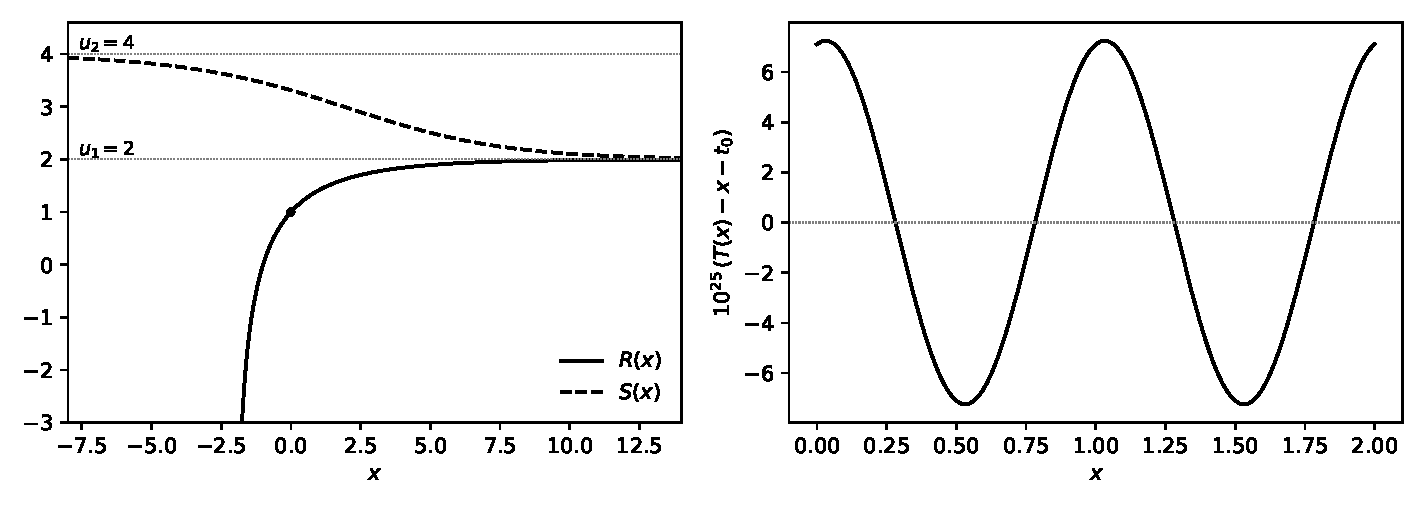
\includegraphics[width=\textwidth]{figures/fig2_regular.pdf}
  \caption{$b=\sqrt2$。左：$R(x)$（实线，$x>-2$）与 $S(x)$（虚线），点为 $R(0)=1$，点线为不动点 $2$、$4$。
  右：转移映射的非常数部分 $10^{25}(T(x)-x-t_0)$，它是实值、1-周期的，振幅 $2|t_1|=7.25\times10^{-25}$（\cref{ch2:ex:sqrt2-transition}）。
  脚本 \texttt{figures/fig2\_regular.py}。}
  \label{ch2:fig:regular}
\end{figure}

% ==================================================================
\section{两个分数次迭代}\label{ch2:sec:two}

由 \cref{prop:regular-periodic}(b)(c)，函数 $x\mapsto R(x+\ii h/2)$ 与 $x\mapsto S(x)$ 都是 $\R$ 到区间 $I=(u_1,u_2)$ 的实解析递减双射，都满足 $F(x+1)=f(F(x))$。
它们是 $f|_I$ 的两个实超函数：一个在 $u_1$ 处正则，一个在 $u_2$ 处正则。

\begin{proposition}\label{ch2:prop:two-abel}
设 $f$ 满足 \textup{(K1)--(K3)}。在 $I=(u_1,u_2)$ 上令
\[
  A_R(u):=R^{-1}(u)-\ii\frac h2=\frac{\log\bigl(\sigma(u)/|\sigma(\ustar)|\bigr)}{\log\lambda_1},\qquad
  A_S(u):=S^{-1}(u)=\frac{\log\bigl(-\sigma_{\mathrm{rep}}(u)\bigr)}{\log\lambda_2}.
\]
\begin{enumerate}[label=(\alph*)]
\item $A_R$ 与 $A_S$ 都是 $f|_I$ 的 Abel 函数，都是 $I$ 到 $\R$ 的实解析递减双射。
\item 存在实解析的 1-周期函数 $\theta$ 使 $A_R=A_S+\theta\circ A_S$。若令 $T(x):=R^{-1}(S(x))$（取 $\Ima T=h/2$ 的分支），则
  \[
    \theta(x)=T(x)-x-\ii\frac h2,\qquad T(x+1)=T(x)+1 .
  \]
\item 两个分数次迭代
  \[
    f_R^{\circ t}:=A_R^{-1}\circ(A_R+t)=\sigma^{-1}\circ(\lambda_1^{\,t}\sigma),\qquad
    f_S^{\circ t}:=A_S^{-1}\circ(A_S+t)=\sigma_{\mathrm{rep}}^{-1}\circ(\lambda_2^{\,t}\sigma_{\mathrm{rep}})
  \]
  （$\sigma^{-1}$、$\sigma_{\mathrm{rep}}^{-1}$ 指 $\sigma|_I$、$\sigma_{\mathrm{rep}}|_I$ 的反函数）
  对一切 $t$ 相同，当且仅当 $T-\id$ 是常数，即 $T$ 的 Fourier 系数 $t_n$（$n\ne0$）全为零。
\end{enumerate}
\end{proposition}

\begin{proof}
(a) 由 \cref{prop:regular-periodic}(e)。Abel 方程：$\sigma(f(u))=\lambda_1\sigma(u)$ 推出 $A_R(f(u))=A_R(u)+1$；$A_S$ 同理。
(b) 令 $\theta:=A_R\circ A_S^{-1}-\id=A_R\circ S-\id$，它是实解析函数的复合。由 $S(x+1)=f(S(x))$ 和 $A_R\circ f=A_R+1$，
$\theta(x+1)=A_R(f(S(x)))-x-1=A_R(S(x))-x=\theta(x)$。于是 $A_R=(\id+\theta)\circ A_S=A_S+\theta\circ A_S$。
$A_R(S(x))=R^{-1}(S(x))-\ii h/2=T(x)-\ii h/2$。$T(x+1)=T(x)+1$ 等价于 $\theta$ 的周期性。
(c) 两个表达式是 Abel 坐标定义的直接改写（$A_R+t$ 对应于 $\sigma$ 乘以 $\lambda_1^{\,t}$）。
记 $\varphi=\id+\theta$，它是 $\R$ 上的递增双射，$f_R^{\circ t}=A_S^{-1}\circ\varphi^{-1}\circ(\varphi\circ A_S+t)$。
所以 $f_R^{\circ t}=f_S^{\circ t}$ 对一切 $t$ 成立，当且仅当 $\varphi(y+t)=\varphi(y)+t$ 对一切 $y,t$ 成立，即 $\theta$ 为常数（第~\ref{ch:intro}~章的不唯一性命题）。
由 (b)，这等价于 $T-\id$ 为常数。
\end{proof}

$T$ 在实轴附近的带形上全纯，$T(z)-z=\sum_{n\in\Z}t_n\ee^{2\pi\ii nz}$；由 $\theta$ 取实值，$t_{-n}=\overline{t_n}$，$\Ima t_0=h/2$。
这是第~\ref{ch:transition}~章 \cref{def:transition} 的转移映射和 \cref{lem:realT} 的实结构。
「$R$ 和 $S$ 是两个不同的分数次迭代」的精确含义是：$T$ 不是平移。
对 Möbius 变换，$T$ 恰好是平移（\cref{ch2:ex:mobius}）；对 $b^w$，$T$ 不是平移，但差别极小：

\begin{example}[$b=\sqrt2$ 的转移映射]\label{ch2:ex:sqrt2-transition}
\texttt{figures/ch02\_sqrt2.py} 在 $16$ 个等距点上计算 $T(x)=R^{-1}(S(x))$，用离散 Fourier 变换求系数（混叠误差来自 $t_{\pm15}$，可以忽略）。结果（数值）：
\[
\begin{aligned}
  t_0&=-5.2840469112759295096+8.5715740896774235521\,\ii,\qquad \Ima t_0=h/2,\\
  t_1&=\overline{t_{-1}}=3.55397489161\times10^{-25}-7.19565846479\times10^{-26}\,\ii,\\
  |t_1|&=3.62608777302\times10^{-25},\qquad |t_2|=2.06254669064\times10^{-49}.
\end{aligned}
\]
因为 $|\ee^{-2\pi\ii t_0}|=\ee^{2\pi\Ima t_0}=\ee^{\pi h}$，$t_n$ 天然地含有因子 $\ee^{-n\pi h}=\Lam^{n/2}$（$\ee^{-\pi h}=4.0766\times10^{-24}$）。
去掉这个因子，得到第~\ref{ch:transition}~章的规范化系数 $\tau_n=t_n\ee^{-2\pi\ii nt_0}$：
\[
\begin{gathered}
  \tau_1=-0.00125909725971+0.0889407535848\,\ii,\\
  |\tau_1|=0.0889496653965,\qquad|\tau_2|=0.01241125793 .
\end{gathered}
\]
两个半迭代在 $u=3$ 处的值是
\[
\begin{aligned}
  f_R^{\circ1/2}(3)&=2.913786734633452607979441747\ldots,\\
  f_S^{\circ1/2}(3)&=2.913786734633452607979441917\ldots,
\end{aligned}
\]
相差 $-1.694\times10^{-25}$。它们在双精度下无法区分，但不相等。
\end{example}

这个例子预告了后面各章的三个结论。
\begin{enumerate}[label=(\arabic*)]
\item \emph{汇流。}第~\ref{ch:confluence}~章证明 $b\to\eta^-$ 时 $\tau_n\to B_n\ee^{2\pi\ii na}$（\cref{thm:confluence}），
  其中 $B_n$ 是抛物芽 $\ee^u-1$ 的逆 horn 映射的系数（\cref{def:horn}），$|B_1|=0.0890584364\ldots$，$|B_2|=0.0124873841\ldots$~\cite[\S2.1]{KneserPaper}。
  $b=\sqrt2$ 离 $\eta=1.44467$ 并不很近，$|\tau_1|$ 与 $|B_1|$ 已相差约 $0.12\%$，$|\tau_2|$ 与 $|B_2|$ 相差约 $0.6\%$。
  相位也接近：$\arg\tau_1=1.584952\ldots$，而极限相位是 $\arg B_1+2\pi a\equiv1.58653\ldots$（模 $2\pi$，\cite[\S2.1]{KneserPaper}）。
\item \emph{尺度。}$t_1$ 的大小 $\approx\ee^{-\pi h}|\tau_1|$ 是指数小的。第~\ref{ch:unfolding}~章证明 $h\sim\pi/\sqrt{a_2\gamma s}$（\cref{prop:scales}），所以这种指数小在鞍结附近是「超越所有阶」的。
\item \emph{缝合。}第~\ref{ch:sewing}~章的缝合解 $\Ksew=R\circ(\id+\sum_{n\ge0}c_n\ee^{2\pi\ii nz})$ 满足 $c_n=\Lam^n\bigl(\tau_n+O(\Lam)\bigr)$（\cref{thm:sewing}，$s$ 充分小时）。
  在 $z=\frac12$ 处，一阶近似给出
  \[
    \Ima\Ksew_{\sqrt2}(\tfrac12)\approx\Ima\bigl(c_1R'(\tfrac12)(\ee^{\ii\pi}-1)\bigr)=-2R'(\tfrac12)\,\Ima(\Lam\tau_1)=-1.18899697185\times10^{-48},
  \]
  其中 $R'(\frac12)=0.40221842463187347989$（同一脚本）。这与 \cite{KneserPaper} 用缝合方程直接算出的 $-1.18899697185\times10^{-48}$ 在所列的 $12$ 位上一致，
  也与 Paulsen 的 $-1.18899697\times10^{-48}$~\cite[\S6]{Paulsen2019} 在所给的 9 位上一致（第~\ref{ch:intro}~章）。
  若 \cref{thm:sewing} 的估计在 $b=\sqrt2$ 处适用，被忽略的项相对大小是 $O(\Lam)\approx10^{-47}$；
  但定理只对充分接近 $\eta$ 的 $b$ 证明，所以这里的一致是数值事实。
\end{enumerate}

% ==================================================================
\notes

\paragraph{Koenigs 定理。}
\cref{thm:koenigs} 属于 G.~Koenigs~\cite{Koenigs1884}。Schröder~\cite{Schroder1870} 在 1870 年研究了 \eqref{ch2:eq:schroder}；形式解（\cref{ch2:lem:formal}）的递推是标准的。
本章的证明（极限 \eqref{ch2:eq:koenigs-limit} 与直接的唯一性论证）沿用~\cite[\S8]{Milnor2006}；另见~\cite[Ch.~II]{CarlesonGamelin1993}。
Poincaré 函数（\cref{ch2:prop:poincare}）以 H.~Poincaré 命名。
关于中性不动点的线性化（Siegel、Brjuno、Cremer）见~\cite[\S11]{Milnor2006}，本书不需要。

\paragraph{正则解与 tetration。}
吸引不动点处的正则迭代是函数方程文献中的标准构造；对 tetration，它就是 $1<b<\eta$ 时通常所说的「正则 tetration」。
Kouznetsov 与 Trappmann~\cite{KouznetsovTrappmann2010} 研究了底数 $\sqrt2$ 的正则超指数，包括在两个不动点 $2$、$4$ 处构造的超指数及其复平面上的图像；
\cref{ch2:ex:four} 的四个实函数可以与之对照。
$S$ 与 $R^{-1}$ 的定义、$\sigma(\ustar)<0$ 的作用以及 \cref{prop:regular-periodic}(e) 的实结构取自~\cite[\S3.1]{KneserPaper}，
那里写的是 tetration（$w_0=1$）；一般开折的改写（用 (H4) 代替 $1<\ee^{\lambda_1}$）见 \texttt{sec-general.tex}。
\cref{ch2:lem:param} 是~\cite[Lemma~2.1]{KneserPaper}。
\cref{ch2:prop:regular-unique} 是第~\ref{ch:intro}~章的不唯一性命题与 Liouville 定理的直接结合；在~\cite{KneserPaper} 中没有单独陈述。

\paragraph{与后面各章的对应。}
本章对固定的 $f$ 讨论问题。第~\ref{ch:unfolding}~章让 $f=f_s$ 依赖参数 $s$，此时 $\lambda_1,\lambda_2\to1$，$h,h_2\to\infty$，$\Lam\to0$；
本章 (K1)--(K3) 由 (H1)--(H4) 对充分小的 $s>0$ 推出。
\cref{ch2:sec:two} 的 $T$ 在第~\ref{ch:transition}~章正式定义（\cref{def:transition}），并且那里把它延拓到实轴下方的一个带形，那是缝合与汇流发生的地方。

% ==================================================================
\exercises

\begin{exercise}\label{ch2:ex:series}
设 $f(z)=\lambda z+z^2$，$0<|\lambda|<1$。用 \eqref{ch2:eq:recursion} 证明 Koenigs 坐标的前几项是
\[
  \sigma(z)=z+\frac{z^2}{\lambda-\lambda^2}+\frac{2\,z^3}{(\lambda-\lambda^2)(1-\lambda^2)}+O(z^4).
\]
分母中出现的 $\lambda-\lambda^k$ 在 $\lambda\to1$ 时趋于零，这预示了抛物情形的困难。
\end{exercise}

\begin{exercise}\label{ch2:ex:eigen}
在 \cref{thm:koenigs} 的条件下，设 $\varphi$ 在 $p$ 附近全纯、不是常数，$\varphi(p)=0$，且 $\varphi\circ f=\mu\varphi$（$\mu\in\C$）。
证明存在正整数 $m$ 和常数 $c\ne0$，使 $\mu=\lambda^m$，$\varphi=c\,\sigma^m$。
\end{exercise}
\begin{hint}
在坐标 $\zeta=\sigma(u)$ 中考虑 $k=\varphi\circ\sigma^{-1}$，它满足 $k(\lambda\zeta)=\mu k(\zeta)$。比较幂级数的各项系数。
\end{hint}

\begin{exercise}\label{ch2:ex:real-branch}
设 $f$ 在实轴上取实值，$p\in\R$ 是吸引不动点，乘子 $0<\lambda<1$。对 $\ell=\log\lambda+2\pi\ii k$（$k\in\Z$）定义 $f^{\circ t}_{(\ell)}=\Psi\circ(\ee^{\ell t}\sigma)$。
证明：对固定的实数 $t$，$f_{(\ell)}^{\circ t}$ 在 $p$ 附近的实轴上取实值，当且仅当 $2kt\in\Z$；所以它对每个实数 $t$ 都取实值，当且仅当 $k=0$。
对 $t=\frac12$ 与奇数 $k$，$f_{(\ell)}^{\circ1/2}=\Psi\circ(-\sqrt\lambda\,\sigma)$ 是实的，它在 $p$ 附近递增还是递减？
\end{exercise}

\begin{exercise}\label{ch2:ex:mobius}
设 $f(u)=u/(2-u)$。它在 $u_1=0$、$u_2=1$ 处有不动点，乘子 $\frac12$ 和 $2$，并且在 $[\ustar,1]$（$\ustar=-\frac12$）上满足 (K3)。$f$ 不是整函数，但 \cref{def:regular-solution} 的公式仍有意义。
\begin{enumerate}[label=(\alph*)]
\item 证明 $\sigma(u)=u/(1-u)$，$\sigma_{\mathrm{rep}}(u)=-(1-u)/u$。
\item 写出 $R$、$S$，并证明 $T=R^{-1}\circ S$ 是平移 $T(z)=z+t_0$。求 $t_0$，并验证 $\Ima t_0=h/2$。
\item 由 \cref{ch2:prop:two-abel}(c) 说明：对这个 $f$，两个正则分数迭代在 $(0,1)$ 上相同。
\end{enumerate}
\end{exercise}
\begin{hint}
$y=u/(1-u)$ 把 $f$ 共轭成 $y\mapsto y/2$，$1/y$ 把 $f$ 共轭成 $y\mapsto 2y$。
\end{hint}

\begin{exercise}\label{ch2:ex:real-lines}
设 $f$ 满足 (K1)--(K3)。证明：对实数 $y$，$R(x+\ii y)$ 对一切充分大的实数 $x$ 取实值，当且仅当 $y\in\frac h2\Z$。
\end{exercise}

\begin{exercise}\label{ch2:ex:bw-domain}
对 $f(w)=b^w$（$1<b<\eta$，$w_0=1$）补全 \cref{ch2:ex:bw-singular} 的细节：证明 $R'(x)>0$ 于 $(-2,\infty)$，$R(-1)=0$，并利用 $R(x)=\log_bR(x+1)$ 证明 $x\downarrow-2$ 时 $R(x)\to-\infty$。
\end{exercise}

\begin{exercise}\label{ch2:ex:four}
对 $f(w)=b^w$（$1<b<\eta$），证明 $x\mapsto S(x+\ii h_2/2)$ 是实值的，严格递增，把 $\R$ 双射到 $(\ee^{\lambda_2},+\infty)$，并满足 $F(x+1)=b^{F(x)}$。
于是得到 $f$ 的四个实超函数：$R$（取值于 $(-\infty,\ee^{\lambda_1})$）、$R(\cdot+\ii h/2)$ 与 $S$（取值于 $(\ee^{\lambda_1},\ee^{\lambda_2})$）、$S(\cdot+\ii h_2/2)$（取值于 $(\ee^{\lambda_2},\infty)$）。
\end{exercise}
\begin{hint}
$-\lambda_2^{\,x+\ii h_2/2}=\lambda_2^{\,x}>0$。证明 $\Psi_2$ 把 $(0,\infty)$ 递增地映到 $(\ee^{\lambda_2},\infty)$：在 $0$ 附近 $\Psi_2'(0)=1>0$，
再用 $\Psi_2(\lambda_2y)=b^{\Psi_2(y)}$ 和 $b^w>w$（$w>\ee^{\lambda_2}$）。
\end{hint}

\begin{exercise}\label{ch2:ex:h2-h}
对 $f(w)=b^w$，令 $\lambda_1=1-\varepsilon$。
\begin{enumerate}[label=(\alph*)]
\item 由 $\lambda_1\ee^{-\lambda_1}=\lambda_2\ee^{-\lambda_2}$ 证明 $\lambda_2=1+\varepsilon+\frac23\varepsilon^2+O(\varepsilon^3)$。
\item 证明 $\frac1{\log\lambda_1}+\frac1{\log\lambda_2}=\frac13+O(\varepsilon)$，从而 $h_2-h\to\frac{2\pi}3$（$b\to\eta^-$）。
\item 用表~\ref{ch2:tab:sqrt2} 检验：$b=\sqrt2$ 时 $h_2-h=2.0930$，$2\pi/3=2.0944$。
\end{enumerate}
\end{exercise}
\begin{hint}
(a) 令 $\lambda_2=1+\delta$，比较 $(1-\varepsilon)\ee^{\varepsilon}=1-\frac{\varepsilon^2}2-\frac{\varepsilon^3}3+O(\varepsilon^4)$ 与 $(1+\delta)\ee^{-\delta}=1-\frac{\delta^2}2+\frac{\delta^3}3+O(\delta^4)$。
(b) $\frac1{\log(1-\varepsilon)}=-\frac1\varepsilon+\frac12+O(\varepsilon)$，$\frac1{\log\lambda_2}=\frac1\varepsilon-\frac16+O(\varepsilon)$。
一般开折的对应结论是 $h_2-h\to2\pi\rho$（\cref{prop:scales}）。
\end{hint}

\begin{exercise}\label{ch2:ex:complex-unique}
（较难）设 $p$ 是吸引不动点，乘子 $\lambda$ 是非实复数，$0<|\lambda|<1$。设 $F$ 在右半平面上全纯，$F(z+1)=f(F(z))$，且 $F(z)\to p$ 关于 $\Ima z$ 一致（$\Rea z\to+\infty$）。
证明 $F\equiv p$ 或存在 $\lambda$ 的一个对数 $\ell$ 和常数 $c\ne0$ 使 $F(z)=\Psi(c\,\ee^{\ell z})$。对数 $\ell$ 的哪些选取能出现？
\end{exercise}
\begin{hint}
固定一个对数 $\ell_0$，令 $\phi=\sigma(F)\ee^{-\ell_0z}$。它是 1-周期的，在带形上满足 $|\phi(x+\ii y)|\le C\ee^{|\Ima\ell_0||y|}$。
Fourier 系数 $\phi_n=\int_0^1\phi(x+\ii y)\ee^{-2\pi\ii n(x+\ii y)}\dd x$ 对每个 $y$ 都成立，令 $y\to\pm\infty$ 估计哪些 $\phi_n$ 可以非零。
再说明若有两个非零系数，$\sigma(F)$ 在某个方向上不趋于 $0$。
\end{hint}

\begin{exercise}\label{ch2:ex:T-monotone}
（较难，预告 \cref{lem:realT}）设 $f$ 满足 (K1)--(K3)，$T(x)=R^{-1}(S(x))$ 取 $\Ima T=h/2$ 的分支。证明 $T'(x)>0$ 对一切实数 $x$ 成立，
并说明为什么这推出 $T$ 在包含实轴的某个水平带内是单射。
\end{exercise}
\begin{hint}
$T'(x)=\dfrac{\sigma'(S(x))\,S'(x)}{\sigma(S(x))\log\lambda_1}$，逐个确定四个因子的符号。单射性：$T(x+1)=T(x)+1$，用紧性论证。
\end{hint}

\begin{exercise}\label{ch2:ex:numerics}
（数值）修改 \texttt{figures/ch02\_sqrt2.py}，对 $b=1.3,\ 1.4,\ 1.44$ 计算 $h$、$|t_1|$ 与 $|\tau_1|$，并与 $|B_1|=0.0890584364\ldots$ 比较。
说明为什么迭代步数 $N$ 必须随 $1/|\log\lambda_1|$ 增长，以及为什么工作精度必须超过 $\pi h/\log10$ 位才能看到 $t_1$。
\end{exercise}
